Se realizo un Modelo de Entidad Relación y Modelo Relacional derivado, los cuales fueron utilizados para implementar la solución. \\

A continuación se muestra el MER realizado:\\

\vspace*{0.3cm} \vspace*{0.3cm}
  \begin{center}
 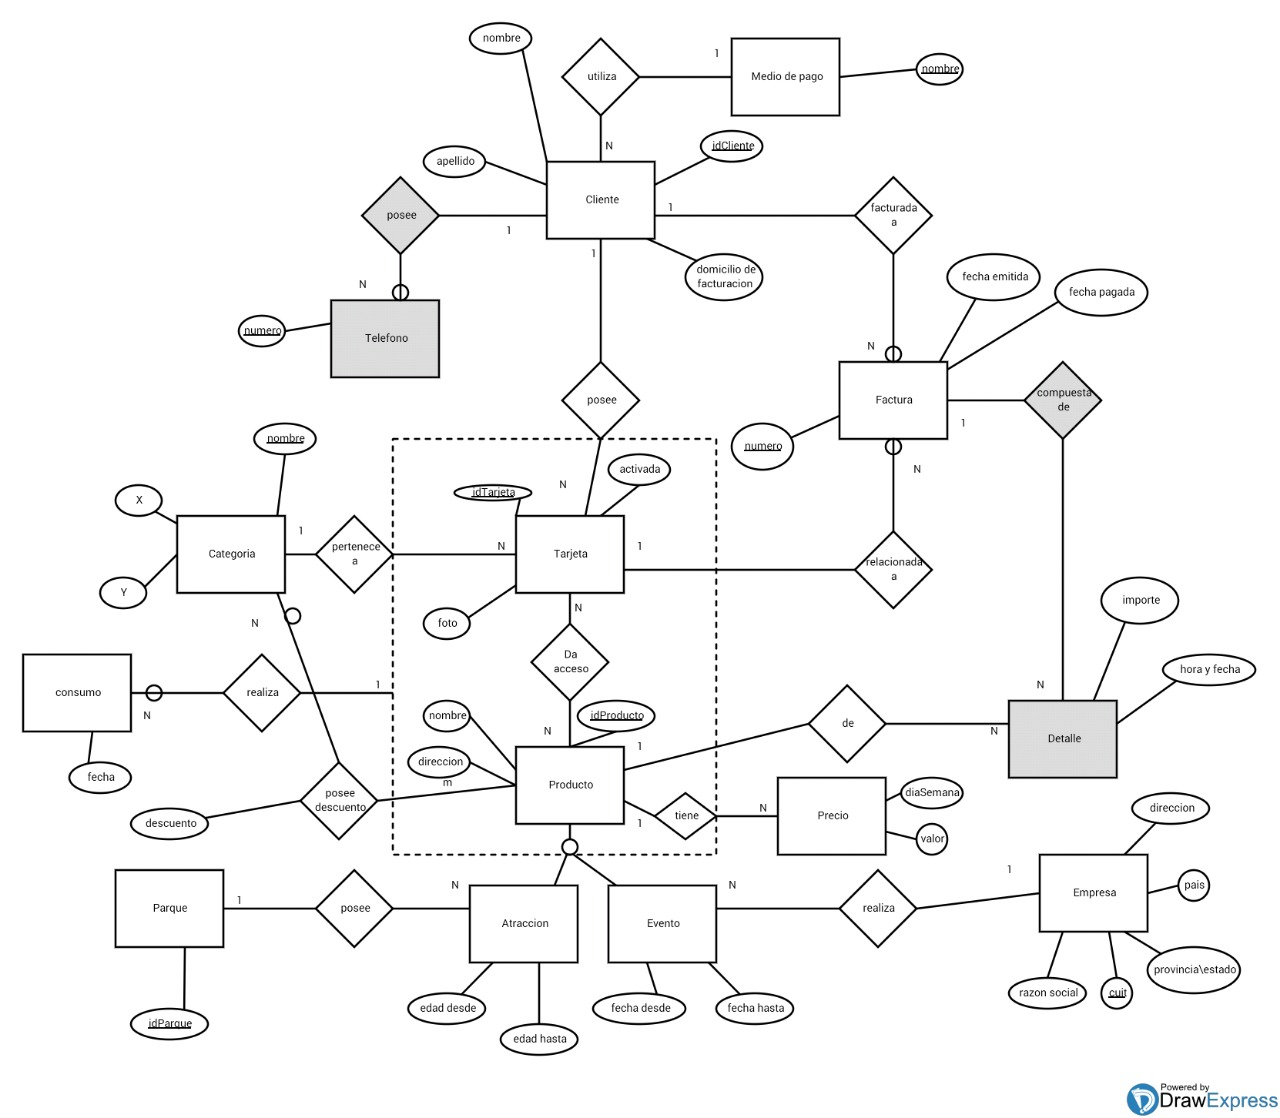
\includegraphics[scale=0.43]{der.jpeg}
 {$Gr$\'a$fico$ $Modelo$ $Entidad$ $Relaci$\'o$n$}
  \end{center}
  \vspace*{0.3cm}
  
En base al MER realizado se derivan las siguientes tablas con sus respectivos atributos y claves:\\

\textbf{Cliente}(\underline{idCliente}, nombre, apellido, domicilioFact)\\
PK =  $\lbrace$idCliente$\rbrace$  \\
\textbf{Telefono}(\underline{idCliente}, telefono)\\
PK = $\lbrace$idCliente, telefono$\rbrace$ FK = $\lbrace$idCliente$\rbrace$\\
\textbf{MedioDePago}(\underline{idCliente, idMedioDePago}, nombre)\\
PK = $\lbrace$idCliente, idMedioDePago$\rbrace$ FK = $\lbrace$idCliente$\rbrace$\\
\textbf{factura}(\underline{tipo, num}, fechaEmitida, fechaVencimiento, medioDePago, nombreCliente)\\
PK = $\lbrace$tipo, num$\rbrace$ \\
\textbf{detalle}(\underline{tipo, num, idDetalle}, importe, horaYFecha, idConsumo)\\
PK = $\lbrace$tipo,num,idDetalle$\rbrace$ FK = $\lbrace$tipo,num$\rbrace$\\
\textbf{recibo}(\underline{tipo, num, idRecibo}, precioPagado)\\
PK = $\lbrace$tipo, num, idRecibo$\rbrace$ FK = $\lbrace$tipo,num$\rbrace$\\
\textbf{Empresa}(\underline{idEmpresa, idProducto}, cuit, razonSocial, pais, direccion, provincia/estado)\\
PK = $\lbrace$idEmpresa, idEvento$\rbrace$ FK = $\lbrace$idEvento$\rbrace$\\
\textbf{Consumo}(\underline{idConsumo}, idProducto, fechaYhora, importe, idTarjeta)\\
PK = $\lbrace$idConsumo$\rbrace$ FK = $\lbrace$idProducto, idTarjeta$\rbrace$\\
\textbf{Tarjeta}(\underline{idTarjeta}, idCliente, activada, foto)\\
PK = $\lbrace$idTarjeta$\rbrace$ FK = $\lbrace$idCliente$\rbrace$\\
\textbf{Categoria}(\underline{idCategoria, idTarjeta}, nombre, x, y)\\
PK = $\lbrace$idCategoria, idTarjeta$\rbrace$ FK = $\lbrace$idTarjeta$\rbrace$\\
\textbf{Producto}(\underline{idProducto}, nombre, direccion)\\
PK = $\lbrace$idProducto$\rbrace$\\
\textbf{Atraccion}(\underline{idProducto}, edadDesde, edadHasta)\\
PK = $\lbrace$idProducto$\rbrace$ FK = $\lbrace$idProducto$\rbrace$\\
\textbf{Evento}(\underline{idProducto}, fechaDesde, fechaHasta)\\
PK = $\lbrace$idProducto$\rbrace$ FK = $\lbrace$idProducto$\rbrace$\\
\textbf{Parque}(\underline{idProducto}, nombre)\\
PK = $\lbrace$idProducto$\rbrace$ FK = $\lbrace$idProducto$\rbrace$\\
\textbf{Precio}(\underline{idPrecio, idProducto}, valor, diaSemana)\\
PK = $\lbrace$idPrecio, idProducto$\rbrace$ FK = $\lbrace$idProducto$\rbrace$\\
\textbf{PoseeDescuento}(\underline{idCategoria, idProducto}, descuento)\\
PK = $\lbrace$idCategoria, idProducto$\rbrace$ FK = $\lbrace$idCategoria, idProducto$\rbrace$\\
\textbf{DaAcceso}(\underline{idTarjeta, idProducto})\\
PK = $\lbrace$idTarjeta, idProducto$\rbrace$ FK = $\lbrace$idTarjeta, idProducto$\rbrace$\\
